\documentclass[aspectratio=169,11pt]{beamer}
\usepackage[T1]{fontenc}
\usepackage[utf8]{inputenc}
\usepackage{tgheros}
\usepackage{amsmath,amssymb}
\usepackage{booktabs,tabularx,array,adjustbox,graphicx}
\definecolor{ink}{HTML}{1A1F2B}
\definecolor{muted}{HTML}{5B6373}
\definecolor{accent}{HTML}{1F4E79}
\definecolor{flag}{HTML}{9B2C2C}
\definecolor{band}{HTML}{F2F4F7}
\setbeamertemplate{navigation symbols}{}
\setbeamercolor{normal text}{fg=ink}
\setbeamercolor{frametitle}{fg=ink}
\setbeamercolor{framesubtitle}{fg=muted}
\setbeamercolor{itemize item}{fg=accent}
\setbeamercolor{itemize subitem}{fg=muted}
\setbeamerfont{frametitle}{series=\bfseries,size=\Large}
\setbeamerfont{framesubtitle}{shape=\itshape,size=\small}
\setbeamertemplate{itemize item}{\small\raisebox{0.1ex}{$\bullet$}}
\setbeamertemplate{itemize subitem}{\small---}
\makeatletter
\setbeamertemplate{frametitle}{%
  \vspace*{0.6em}\usebeamerfont{frametitle}\usebeamercolor[fg]{frametitle}\insertframetitle\par
  \vspace*{0.25em}{\color{accent}\rule{\linewidth}{0.6pt}}\par
  \ifx\insertframesubtitle\@empty\else{\usebeamerfont{framesubtitle}\usebeamercolor[fg]{framesubtitle}\insertframesubtitle\par}\fi}
\makeatother
\setbeamertemplate{footline}{\hfill{\scriptsize\color{muted}\insertframenumber\,/\,\inserttotalframenumber}\hspace*{1.2em}\vspace*{0.8em}}
\newcolumntype{Y}{>{\raggedright\arraybackslash}X}
\setlength{\tabcolsep}{4pt}
\renewcommand{\arraystretch}{1.15}
\newcommand{\slidenote}[1]{\vfill\parbox{0.9\textwidth}{\scriptsize\itshape\color{flag}#1}\par}

\title{Assessing Legal Meaning Preservation in English and Hindi Simplifications of Indian Statutes Extending JUDGEBERT (EMNLP 2025) from French insurance text to Indian statutes}
\author{Karan Singh, Atharv Arora, Jatin Khanchi}
\institute{Bennett University, Greater Noida, India\\[0.3em]CSET 346 Natural Language Processing (project PID-08), instructor Dr. Surabhi Solanki}
\date{}
\begin{document}
\begin{frame}[plain]
\titlepage
\end{frame}

\begin{frame}{The problem}
\framesubtitle{Simplifying the law is useful; measuring whether the law survived is the hard part}
\small
\begin{itemize}
\item Plain-language statutes widen access to justice — LLMs can rewrite them at scale.
\item But a fluent simplification can drop a proviso, flip an obligation into a permission, or change a deadline.
\item Generic metrics reward overlap, so they miss exactly these changes:
\begin{itemize}\small
\item On FrJUDGE: BERTScore r = 0.46, SBERT r = 0.13 vs. human LMP judgement.
\item BERTScore and MeaningBERT over-score the human label on 82\% of pairs.
\end{itemize}
\item Legal meaning preservation is a separate target that has to be learned.
\end{itemize}
\end{frame}

\begin{frame}{What JUDGEBERT leaves open}
\framesubtitle{Each gap below becomes one of our contributions}
\begin{itemize}
\item French only, one domain (Quebec property-damage insurance), 297 pairs.
\item One simplification style \ensuremath{\rightarrow} narrow label range.
\item Krippendorff's \ensuremath{\alpha} = 0.10: annotators split into lenient and strict groups.
\item Pair-level splits: a test original can reappear in training as an identical DA pair.
\item Its headline 0.97 Pearson is measured on a test set containing trivial identical / unrelated pairs.
\item No out-of-domain test.
\end{itemize}
\end{frame}

\begin{frame}{Our extension}
\small
\begin{itemize}
\item English + Hindi, two Indian central acts: RTI 2005 (public information) and Consumer Protection 2019 (consumer law).
\item Official Hindi is a translation of the same provision \ensuremath{\rightarrow} the language comparison is controlled, not confounded.
\item Three variants per clause: normal (BLESS prompt), aggressive (“explain to a 12-year-old”), perturbed (one additional injected legal error of a known type).
\item Perturbed = a labelled diagnostic set: which legal error types is a metric blind to?
\item Clause-grouped splits, asserted disjoint at clause and text level; sanity checks on holdout provisions used nowhere else.
\end{itemize}
\end{frame}

\begin{frame}{Dataset and provenance}
\framesubtitle{India Code was unreachable, so we used other official government sources and recorded exactly which}
\begin{adjustbox}{max width=\textwidth, max totalheight=0.62\textheight, center}
\begin{minipage}{\textwidth}\footnotesize
\begin{tabularx}{\textwidth}{>{\raggedright\arraybackslash\hsize=1.500\hsize}X>{\raggedright\arraybackslash\hsize=1.500\hsize}X>{\centering\arraybackslash\hsize=0.500\hsize}X>{\centering\arraybackslash\hsize=0.500\hsize}X}
\toprule
\textbf{Document} & \textbf{Edition} & \textbf{Sections} & \textbf{Units} \\
\midrule
RTI Act 2005, English (DoPT) & As on 18 Nov 2025; includes the 2023 amendment & 31 & 109 \\
RTI Act 2005, Hindi (DoPT) & Carries the 2019 amendments; sec. 8(1) is the older wording; text layer unusable, read by OCR (Tesseract 5.4, tessdata\_best hin) & 27 & 101 \\
Consumer Protection Act 2019, English (Gazette) & Act 35 of 2019, 9 Aug 2019; original enactment & 107 & 229 \\
Consumer Protection Act 2019, Hindi & Not used: unavailable when the corpus was built (Bill text as introduced found later) & -- & -- \\
\bottomrule
\end{tabularx}
\end{minipage}
\end{adjustbox}
\slidenote{Consequences: E2 (EN vs HI) is RTI-only; CPA is English-only. The two RTI editions differ at section 8(1) — affected clauses are dropped, never edited.}
\end{frame}

\begin{frame}{The Hindi text layer: a trap worth reporting}
\footnotesize
\begin{itemize}
\item The Hindi PDF is not scanned — but its text layer is unusable, in two different ways.
\item pdftotext: 4.9\% of all Devanagari characters come out as U+FFFD (2461 chars, 100 of 102 units) — irreversible loss.
\item PyMuPDF: nothing lost, but legacy Mangal glyphs land in the Vedic/Sundanese Unicode blocks (2681 chars, 48 distinct code points) and vowel signs are in visual order.
\item Readable to a human, systematically wrong to a machine; no downstream metric would reveal it. So extraction has a quantitative acceptance test and refuses both routes.
\item Fix: OCR at 300 dpi, Tesseract 5.4 + tessdata\_best hin \ensuremath{\rightarrow} Devanagari 0.993, bad-matra 0.000, zero replacement characters.
\item Residual OCR defect: the digit 1 is dropped (12\ensuremath{\rightarrow}“2”, 13\ensuremath{\rightarrow}“03”, “(1)”\ensuremath{\rightarrow}“()”). Numbering is repaired from the sequence, never from appearance; every repair logged.
\end{itemize}
\slidenote{Open item: a Hindi legal reader has not yet verified the OCR'd clauses.}
\end{frame}

\begin{frame}{What the corpus actually contains}
\framesubtitle{78 clauses \ensuremath{\rightarrow} 113 clause-language items \ensuremath{\rightarrow} 338 pairs (RTI 38, of which 35 bilingual; CPA 40, English-only)}
\begin{adjustbox}{max width=\textwidth, max totalheight=0.62\textheight, center}
\begin{minipage}{\textwidth}\footnotesize
\begin{tabularx}{\textwidth}{>{\raggedright\arraybackslash\hsize=1.235\hsize}X>{\raggedright\arraybackslash\hsize=1.235\hsize}X>{\centering\arraybackslash\hsize=0.882\hsize}X>{\centering\arraybackslash\hsize=0.882\hsize}X>{\centering\arraybackslash\hsize=0.882\hsize}X>{\centering\arraybackslash\hsize=0.882\hsize}X}
\toprule
\textbf{Act} & \textbf{Lang} & \textbf{Clauses} & \textbf{Pairs} & \textbf{Mean words} & \textbf{Mean label} \\
\midrule
CPA & EN & 40 & 119 & 50.2 & 7.40 \\
RTI & EN & 38 & 114 & 53.0 & 7.69 \\
RTI & HI & 35 & 105 & 52.5 & 7.49 \\
All &  & 78 & 338 & 51.9 & 7.53 \\
\bottomrule
\end{tabularx}
\end{minipage}
\end{adjustbox}
\slidenote{Clause review was performed by a rule-based agent, not a human, and is disclosed as such; the only text edits permitted were OCR number repairs.}
\end{frame}

\begin{frame}{Scoring protocol — and an honest deviation}
\footnotesize
\begin{itemize}
\item Rubric unchanged from JUDGEBERT: bracket (Accurate 7–10 / Imprecise 2–6 / Off-track 1), minus one point per error, floor 1.
\item Intended: 3 human annotators per pair after a calibration round.
\item Actual, because of the deadline: \textbf{two disclosed LLM annotators}, both Claude Opus 5.5 instances — one model family, not two. One of them also wrote the simplifications, so it is not blind in practice.
\begin{itemize}\footnotesize
\item \ensuremath{\alpha} = 0.610 interval / 0.503 bracket; inter-LLM Pearson 0.723 (agreement, not a ceiling) — vs. \ensuremath{\alpha} = 0.10 between FrJUDGE's five law students. Two instances of one model agreeing is the weaker result. Mean scores differ (8.1 vs 6.9); 68 disagreements unadjudicated.
\end{itemize}
\item Blinding is partial: opaque pair ids and per-annotator shuffle, but annotator A wrote the simplifications; the score is recomputed by our code from bracket + error counts.
\item Human validation: 30-pair blind sheets for the three authors (results reported when scored). The brief's 300 human-judged pairs are not met.
\end{itemize}
\slidenote{Labels in this version are disclosed LLM judgements (two Claude Opus 5.5 instances) under the human rubric — not human legal judgement.}
\end{frame}

\begin{frame}{Method}
\footnotesize
\begin{itemize}
\item LMP model: cross-encoder regression, original [SEP] simplification \ensuremath{\rightarrow} score in 1–10, MSE loss; linear decay, grad clip 1.0, best dev checkpoint.
\begin{itemize}\footnotesize
\item We depart from JUDGEBERT's lr 5e-5 / batch 16 / patience 5: on our \textasciitilde{}35-pair dev split early stopping fired on noise and left the model at the label mean (r \ensuremath{\approx} 0). We use lr 2e-5, batch 8, 30 epochs, no early stopping — disclosed, with the dev-set selection it implies.
\end{itemize}
\item Backbones: XLM-R and MuRIL (IndicBERT v2 planned, not run) — with and without data augmentation, 3 clause-grouped seeds (42–44).
\item Principal system fixed in advance: XLM-R pre-trained on FrJUDGE, fine-tuned with DA.
\item Baselines: ROUGE-L and BLEU (Devanagari-aware tokeniser), LaBSE cosine, multilingual BERTScore F1. No LLM judge: it would be scored against LLM labels (circular).
\item Every baseline mapped to 1–10 twice: naive and train-calibrated.
\item Report Pearson, Spearman, RMSE, MAE and the over-scoring rate — the dangerous failure is flattering a simplification that lost a condition.
\end{itemize}
\end{frame}

\begin{frame}{Experiments E1–E5}
\small
\begin{itemize}
\item E1  Generic similarity baselines vs. the trained LMP models.
\item E2  English vs. Hindi on the 35 RTI clauses present in both languages, and zero-shot EN\ensuremath{\rightarrow}HI / HI\ensuremath{\rightarrow}EN.
\item E3  Cross-act generalisation: train on one act, test on the other (no test-act text in training, including augmentation partners).
\item E4  Sanity checks on disjoint holdouts: identical pairs \ensuremath{\geq} 9.9, unrelated \ensuremath{\leq} 1.1.
\item E5  \ensuremath{\geq} 15 legally difficult cases, grouped by injected error type and recorded change.
\item One command regenerates every table in the paper from the run files.
\end{itemize}
\end{frame}

\begin{frame}{E1: baselines vs. LMP model}
\begin{adjustbox}{max width=\textwidth, max totalheight=0.62\textheight, center}
\begin{minipage}{\textwidth}\tiny
\begin{tabularx}{\textwidth}{>{\raggedright\arraybackslash\hsize=1.588\hsize}X>{\centering\arraybackslash\hsize=0.882\hsize}X>{\centering\arraybackslash\hsize=0.882\hsize}X>{\centering\arraybackslash\hsize=0.882\hsize}X>{\centering\arraybackslash\hsize=0.882\hsize}X>{\centering\arraybackslash\hsize=0.882\hsize}X}
\toprule
\textbf{System} & \textbf{Pearson} & \textbf{Spearman} & \textbf{RMSE} & \textbf{MAE} & \textbf{Over-score \%} \\
\midrule
XLM-R, FrJUDGE\ensuremath{\rightarrow}\allowbreak{}ours, DA & 0.576 \ensuremath{\pm} 0.102 & 0.544 \ensuremath{\pm} 0.106 & 2.037 \ensuremath{\pm} 0.142 & 1.474 \ensuremath{\pm} 0.213 & 38.8 \ensuremath{\pm} 3.9 \\
XLM-R, FrJUDGE\ensuremath{\rightarrow}\allowbreak{}ours, no DA & 0.586 \ensuremath{\pm} 0.098 & 0.553 \ensuremath{\pm} 0.101 & 2.037 \ensuremath{\pm} 0.110 & 1.525 \ensuremath{\pm} 0.042 & 46.1 \ensuremath{\pm} 7.0 \\
XLM-R from scratch, DA & 0.228 \ensuremath{\pm} 0.288 & 0.259 \ensuremath{\pm} 0.280 & 2.464 \ensuremath{\pm} 0.224 & 2.020 \ensuremath{\pm} 0.469 & 47.9 \ensuremath{\pm} 12.1 \\
XLM-R from scratch, no DA & -0.030 \ensuremath{\pm} 0.048 & -0.020 \ensuremath{\pm} 0.044 & 2.444 \ensuremath{\pm} 0.090 & 2.245 \ensuremath{\pm} 0.079 & 45.8 \ensuremath{\pm} 5.6 \\
MuRIL from scratch, DA & 0.067 \ensuremath{\pm} 0.097 & 0.097 \ensuremath{\pm} 0.060 & 2.607 \ensuremath{\pm} 0.180 & 2.365 \ensuremath{\pm} 0.135 & 41.7 \ensuremath{\pm} 6.6 \\
MuRIL from scratch, no DA & -0.042 \ensuremath{\pm} 0.014 & -0.034 \ensuremath{\pm} 0.028 & 4.443 \ensuremath{\pm} 0.058 & 3.876 \ensuremath{\pm} 0.084 & 6.4 \ensuremath{\pm} 2.1 \\
labse-cal & 0.101 \ensuremath{\pm} 0.026 & 0.224 \ensuremath{\pm} 0.066 & 2.417 \ensuremath{\pm} 0.124 & 2.184 \ensuremath{\pm} 0.090 & 44.4 \ensuremath{\pm} 4.8 \\
labse & 0.101 \ensuremath{\pm} 0.026 & 0.224 \ensuremath{\pm} 0.066 & 2.811 \ensuremath{\pm} 0.157 & 2.110 \ensuremath{\pm} 0.121 & 41.0 \ensuremath{\pm} 3.6 \\
bertscore-cal & 0.055 \ensuremath{\pm} 0.040 & 0.115 \ensuremath{\pm} 0.033 & 2.427 \ensuremath{\pm} 0.120 & 2.206 \ensuremath{\pm} 0.088 & 44.7 \ensuremath{\pm} 4.9 \\
bertscore & 0.055 \ensuremath{\pm} 0.040 & 0.115 \ensuremath{\pm} 0.033 & 2.974 \ensuremath{\pm} 0.235 & 2.180 \ensuremath{\pm} 0.232 & 59.2 \ensuremath{\pm} 1.6 \\
bleu-cal & 0.018 \ensuremath{\pm} 0.021 & 0.088 \ensuremath{\pm} 0.042 & 2.433 \ensuremath{\pm} 0.120 & 2.212 \ensuremath{\pm} 0.087 & 45.4 \ensuremath{\pm} 5.8 \\
bleu & 0.018 \ensuremath{\pm} 0.021 & 0.088 \ensuremath{\pm} 0.042 & 5.512 \ensuremath{\pm} 0.238 & 4.977 \ensuremath{\pm} 0.316 & 6.4 \ensuremath{\pm} 1.3 \\
rougeL-cal & 0.010 \ensuremath{\pm} 0.033 & 0.071 \ensuremath{\pm} 0.040 & 2.430 \ensuremath{\pm} 0.119 & 2.217 \ensuremath{\pm} 0.090 & 45.4 \ensuremath{\pm} 5.8 \\
rougeL & 0.010 \ensuremath{\pm} 0.033 & 0.071 \ensuremath{\pm} 0.040 & 4.041 \ensuremath{\pm} 0.159 & 3.563 \ensuremath{\pm} 0.169 & 21.2 \ensuremath{\pm} 1.8 \\
Variant-mean lookup (uses answer key; diagnostic, not a system) & 0.831 \ensuremath{\pm} 0.063 & n/a & 1.385 \ensuremath{\pm} 0.138 & 0.868 \ensuremath{\pm} 0.045 & 33.7 \ensuremath{\pm} 16.7 \\
\bottomrule
\end{tabularx}
\end{minipage}
\end{adjustbox}
\slidenote{Every cell is produced by modeling/evaluate.py from the prediction files. The last row is a diagnostic that uses the answer key, not a system.}
\end{frame}

\begin{frame}{E2: English vs. Hindi on the 35 bilingual RTI clauses}
\begin{adjustbox}{max width=\textwidth, max totalheight=0.62\textheight, center}
\begin{minipage}{\textwidth}\scriptsize
\begin{tabularx}{\textwidth}{>{\raggedright\arraybackslash\hsize=1.452\hsize}X>{\raggedright\arraybackslash\hsize=1.613\hsize}X>{\centering\arraybackslash\hsize=0.645\hsize}X>{\centering\arraybackslash\hsize=0.645\hsize}X>{\centering\arraybackslash\hsize=0.645\hsize}X}
\toprule
\textbf{System} & \textbf{Setting} & \textbf{Pearson} & \textbf{RMSE} & \textbf{Over-score \%} \\
\midrule
XLM-R, FrJUDGE\ensuremath{\rightarrow}\allowbreak{}ours, DA & train EN+HI, test EN & 0.165 \ensuremath{\pm} 0.063 & 2.380 \ensuremath{\pm} 0.161 & 36.7 \ensuremath{\pm} 8.8 \\
XLM-R, FrJUDGE\ensuremath{\rightarrow}\allowbreak{}ours, DA & train EN+HI, test HI & -0.041 \ensuremath{\pm} 0.144 & 2.638 \ensuremath{\pm} 0.334 & 45.6 \ensuremath{\pm} 3.8 \\
XLM-R, FrJUDGE\ensuremath{\rightarrow}\allowbreak{}ours, DA & train EN \ensuremath{\rightarrow}\allowbreak{} test HI (zero-shot) & 0.035 \ensuremath{\pm} 0.027 & 2.564 \ensuremath{\pm} 0.293 & 42.2 \ensuremath{\pm} 1.9 \\
XLM-R, FrJUDGE\ensuremath{\rightarrow}\allowbreak{}ours, DA & train HI \ensuremath{\rightarrow}\allowbreak{} test EN (zero-shot) & 0.131 \ensuremath{\pm} 0.115 & 2.519 \ensuremath{\pm} 0.282 & 31.1 \ensuremath{\pm} 6.9 \\
XLM-R from scratch, DA & train EN+HI, test EN & -0.059 \ensuremath{\pm} 0.197 & 2.391 \ensuremath{\pm} 0.141 & 38.9 \ensuremath{\pm} 7.7 \\
XLM-R from scratch, DA & train EN+HI, test HI & -0.058 \ensuremath{\pm} 0.108 & 2.314 \ensuremath{\pm} 0.146 & 46.7 \ensuremath{\pm} 3.3 \\
XLM-R from scratch, DA & train EN \ensuremath{\rightarrow}\allowbreak{} test HI (zero-shot) & -0.059 \ensuremath{\pm} 0.086 & 2.583 \ensuremath{\pm} 0.315 & 44.4 \ensuremath{\pm} 3.8 \\
XLM-R from scratch, DA & train HI \ensuremath{\rightarrow}\allowbreak{} test EN (zero-shot) & 0.028 \ensuremath{\pm} 0.027 & 2.433 \ensuremath{\pm} 0.074 & 37.8 \ensuremath{\pm} 6.9 \\
\bottomrule
\end{tabularx}
\end{minipage}
\end{adjustbox}
\slidenote{About 126 training pairs per split: too few to show cross-lingual transfer either way.}
\end{frame}

\begin{frame}{E3: train on one act, test on the other}
\begin{adjustbox}{max width=\textwidth, max totalheight=0.62\textheight, center}
\begin{minipage}{\textwidth}\footnotesize
\begin{tabularx}{\textwidth}{>{\raggedright\arraybackslash\hsize=1.692\hsize}X>{\raggedright\arraybackslash\hsize=1.053\hsize}X>{\centering\arraybackslash\hsize=0.752\hsize}X>{\centering\arraybackslash\hsize=0.752\hsize}X>{\centering\arraybackslash\hsize=0.752\hsize}X}
\toprule
\textbf{System} & \textbf{Split} & \textbf{Pearson} & \textbf{RMSE} & \textbf{MAE} \\
\midrule
XLM-R, FrJUDGE\ensuremath{\rightarrow}\allowbreak{}ours, DA & CPA \ensuremath{\rightarrow}\allowbreak{} RTI & 0.388 \ensuremath{\pm} 0.021 & 2.391 \ensuremath{\pm} 0.101 & 1.703 \ensuremath{\pm} 0.031 \\
XLM-R, FrJUDGE\ensuremath{\rightarrow}\allowbreak{}ours, DA & RTI \ensuremath{\rightarrow}\allowbreak{} CPA & 0.119 \ensuremath{\pm} 0.051 & 2.629 \ensuremath{\pm} 0.068 & 2.212 \ensuremath{\pm} 0.041 \\
XLM-R from scratch, DA & CPA \ensuremath{\rightarrow}\allowbreak{} RTI & 0.186 \ensuremath{\pm} 0.053 & 2.603 \ensuremath{\pm} 0.163 & 2.042 \ensuremath{\pm} 0.162 \\
XLM-R from scratch, DA & RTI \ensuremath{\rightarrow}\allowbreak{} CPA & 0.056 \ensuremath{\pm} 0.110 & 2.589 \ensuremath{\pm} 0.036 & 2.299 \ensuremath{\pm} 0.069 \\
\bottomrule
\end{tabularx}
\end{minipage}
\end{adjustbox}
\slidenote{Augmentation partners come only from the training act.}
\end{frame}

\begin{frame}{E4: sanity checks on disjoint holdouts}
\begin{adjustbox}{max width=\textwidth, max totalheight=0.62\textheight, center}
\begin{minipage}{\textwidth}\scriptsize
\begin{tabularx}{\textwidth}{>{\raggedright\arraybackslash\hsize=1.207\hsize}X>{\centering\arraybackslash\hsize=0.862\hsize}X>{\centering\arraybackslash\hsize=0.862\hsize}X>{\centering\arraybackslash\hsize=0.862\hsize}X>{\raggedright\arraybackslash\hsize=1.207\hsize}X}
\toprule
\textbf{System} & \textbf{Identical \ensuremath{\geq} 9.9 \%: EN (n=50)} & \textbf{Identical \ensuremath{\geq} 9.9 \%: HI (n=3)} & \textbf{Unrelated \ensuremath{\leq} 1.1 \%: EN (n=17)} & \textbf{Unrelated \ensuremath{\leq} 1.1 \%: HI (n=0)} \\
\midrule
XLM-R, FrJUDGE\ensuremath{\rightarrow}\allowbreak{}ours, DA & 66.7 \ensuremath{\pm} 57.7 & 66.7 \ensuremath{\pm} 57.7 & 94.1 \ensuremath{\pm} 5.9 & not evaluated \\
XLM-R, FrJUDGE\ensuremath{\rightarrow}\allowbreak{}ours, no DA & 91.3 \ensuremath{\pm} 5.0 & 66.7 \ensuremath{\pm} 0.0 & 17.6 \ensuremath{\pm} 10.2 & not evaluated \\
XLM-R from scratch, DA & 33.3 \ensuremath{\pm} 57.7 & 33.3 \ensuremath{\pm} 57.7 & 31.4 \ensuremath{\pm} 27.8 & not evaluated \\
labse-cal & 0.0 \ensuremath{\pm} 0.0 & 0.0 \ensuremath{\pm} 0.0 & 0.0 \ensuremath{\pm} 0.0 & not evaluated \\
labse & 100.0 \ensuremath{\pm} 0.0 & 100.0 \ensuremath{\pm} 0.0 & 0.0 \ensuremath{\pm} 0.0 & not evaluated \\
bertscore & 100.0 \ensuremath{\pm} 0.0 & 100.0 \ensuremath{\pm} 0.0 & 0.0 \ensuremath{\pm} 0.0 & not evaluated \\
bleu & 100.0 \ensuremath{\pm} 0.0 & 100.0 \ensuremath{\pm} 0.0 & 11.8 \ensuremath{\pm} 0.0 & not evaluated \\
rougeL & 100.0 \ensuremath{\pm} 0.0 & 100.0 \ensuremath{\pm} 0.0 & 0.0 \ensuremath{\pm} 0.0 & not evaluated \\
\bottomrule
\end{tabularx}
\end{minipage}
\end{adjustbox}
\slidenote{JUDGEBERT-DA was the only metric in the original study to pass both checks.}
\end{frame}

\begin{frame}{Within each variant (principal system, E1)}
\begin{adjustbox}{max width=\textwidth, max totalheight=0.62\textheight, center}
\begin{minipage}{\textwidth}\footnotesize
\begin{tabularx}{\textwidth}{>{\raggedright\arraybackslash\hsize=1.312\hsize}X>{\centering\arraybackslash\hsize=0.938\hsize}X>{\centering\arraybackslash\hsize=0.938\hsize}X>{\centering\arraybackslash\hsize=0.938\hsize}X>{\centering\arraybackslash\hsize=0.938\hsize}X>{\centering\arraybackslash\hsize=0.938\hsize}X}
\toprule
\textbf{Variant} & \textbf{n per test split} & \textbf{Mean label} & \textbf{MAE XLM-R, FrJUDGE\ensuremath{\rightarrow}\allowbreak{}ours, DA} & \textbf{Mean signed error XLM-R, FrJUDGE\ensuremath{\rightarrow}\allowbreak{}ours, DA} & \textbf{Within-variant Pearson XLM-R, FrJUDGE\ensuremath{\rightarrow}\allowbreak{}ours, DA} \\
\midrule
normal & 33 \ensuremath{\pm} 1 & 9.96 \ensuremath{\pm} 0.02 & 1.015 \ensuremath{\pm} 0.630 & -0.995 \ensuremath{\pm} 0.640 & 0.314 \ensuremath{\pm} 0.363 \\
aggressive & 33 \ensuremath{\pm} 1 & 7.64 \ensuremath{\pm} 0.27 & 1.205 \ensuremath{\pm} 0.134 & -0.683 \ensuremath{\pm} 0.294 & 0.487 \ensuremath{\pm} 0.063 \\
perturbed & 33 \ensuremath{\pm} 1 & 5.04 \ensuremath{\pm} 0.60 & 2.203 \ensuremath{\pm} 0.057 & 1.961 \ensuremath{\pm} 0.189 & 0.584 \ensuremath{\pm} 0.047 \\
\bottomrule
\end{tabularx}
\end{minipage}
\end{adjustbox}
\slidenote{A variant-mean lookup reaches 0.831 overall, so overall Pearson mostly rewards telling variants apart; within-variant Pearson is the more honest measure.}
\end{frame}

\begin{frame}{Two traps that silently ruin results}
\small
\begin{itemize}
\item transformers 5.x loads CamemBERT-v2 through the auto-tokenizer as a byte-level tokenizer with no merges \ensuremath{\rightarrow} single-character tokens.
\begin{itemize}\small
\item Pairs became \textasciitilde{}650 tokens, were truncated, and training collapsed to predicting the label mean (train MSE \ensuremath{\approx} label variance; test r \ensuremath{\approx} \ensuremath{-}0.25). Nothing errored.
\end{itemize}
\item The Hindi extraction failure above: two extractors, two silent corruptions.
\item Both are now detected in code, and we report them because neither announces itself.
\item FrJUDGE reproduction as an end-to-end check of the training code: 0.707 \ensuremath{\pm} 0.042 Pearson / 1.79 RMSE over 10 seeds vs. published 0.74 \ensuremath{\pm} 0.02 / 1.72.
\end{itemize}
\end{frame}

\begin{frame}{Demo: score, decision and likely legal error}
\begin{itemize}
\item Live app with the MuRIL score model (test Pearson \textbf{0.682}) and MuRIL error classifier (macro-F1 \textbf{0.826}).
\item Per pair: LMP score 1–10, decision, likely legal error with an explanation, rule-based cue check.
\item Below: test pair cpa-s10\_1, where \emph{shall … establish} became \emph{will not set up} (reference 2.5, dotted mark).
\end{itemize}
\vspace{0.6em}
\begin{center}
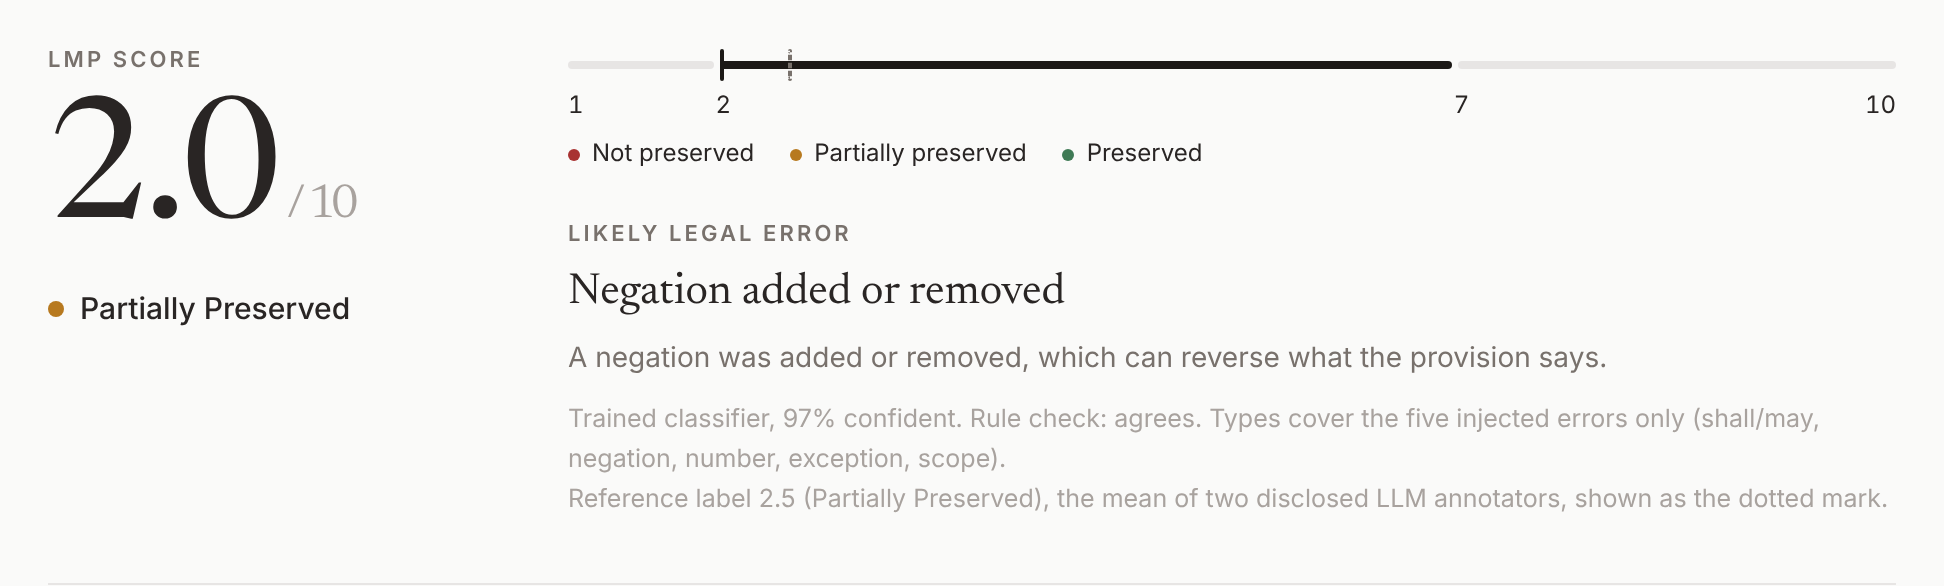
\includegraphics[width=0.68\textwidth]{figures/slide17_1.png}
\end{center}
\slidenote{A prediction, not an annotation. Obligation \ensuremath{\leftrightarrow} permission flips (must \ensuremath{\rightarrow} may) can still score 10; the error classifier usually names them. The app states it is not fit for legal use.}
\end{frame}

\begin{frame}{Trained on our corpus alone, it is unstable}
\framesubtitle{\textasciitilde{}200 training pairs per split}
\small
\begin{itemize}
\item Best from-scratch metric: XLM-R + DA, Pearson \textbf{0.228 \ensuremath{\pm} 0.288} (seeds 0.56 / 0.08 / 0.05). The SD exceeds the mean.
\begin{itemize}\small
\item \ensuremath{\approx} 1.4 standard errors from zero: not distinguishable from no correlation, nor from calibrated LaBSE at 0.101.
\end{itemize}
\item Without DA: \ensuremath{-}0.030. MuRIL + DA: 0.067; MuRIL without DA collapses (RMSE 4.4).
\item The same code reaches \textbf{0.707 on FrJUDGE}, which is consistent with too little data — but FrJUDGE also differs in language, domain and label spread, so this is not proof.
\end{itemize}
\end{frame}

\begin{frame}{Pre-training on FrJUDGE helps, and stabilises}
\framesubtitle{French insurance forms \ensuremath{\rightarrow} Indian statutes in English and Hindi}
\footnotesize
\begin{itemize}
\item Pre-train the same cross-encoder on \textbf{FrJUDGE} (0.85–0.87 on its test set), then fine-tune on our Indian splits.
\item Principal system (with DA): \textbf{Pearson 0.576 \ensuremath{\pm} 0.102} (seeds 0.564 / 0.684 / 0.481); without DA 0.586 \ensuremath{\pm} 0.098 — within noise. From scratch: 0.228 \ensuremath{\pm} 0.288.
\begin{itemize}\footnotesize
\item Transferred seeds lie in 0.48–0.68; from-scratch seeds in 0.05–0.56.
\end{itemize}
\item \textbf{Per language (E1):} EN 0.297 \ensuremath{\rightarrow} \textbf{0.675}, HI 0.010 \ensuremath{\rightarrow} \textbf{0.308} — confounded by act (EN pools both acts; same runs: CPA 0.669 vs RTI 0.485).
\item \textbf{Across acts (E3):} CPA\ensuremath{\rightarrow}RTI 0.186 \ensuremath{\rightarrow} \textbf{0.388}, RTI\ensuremath{\rightarrow}CPA 0.056 \ensuremath{\rightarrow} \textbf{0.119}. Asymmetric.
\item \textbf{E2 (35 bilingual clauses):} joint training EN 0.165, HI \ensuremath{-}0.041; zero-shot EN\ensuremath{\rightarrow}HI 0.035, HI\ensuremath{\rightarrow}EN 0.131. Inconclusive: too little data to tell a language gap from a data gap.
\end{itemize}
\slidenote{Principal system chosen after E1 was known (mirrors JUDGEBERT-DA). Not evidence that LMP is language-independent: LLM labels, and E2 shows no transfer.}
\end{frame}

\begin{frame}{What the diagnostics show}
\footnotesize
\begin{itemize}
\item \textbf{The corpus encodes its construction.} A variant-mean lookup (uses the answer key) reaches \textbf{0.831} — above every model. Within each variant the principal system still correlates \textbf{0.49} (aggressive) and \textbf{0.58} (perturbed).
\item \textbf{Negation vs. modality.} Calibrated LaBSE's hardest error is negation (MAE \textbf{4.63} vs \textasciitilde{}2.3–2.7 elsewhere). The principal system handles negation (\textbf{1.90}); its weak point is shall\ensuremath{\rightarrow}may modality (\textbf{3.16}).
\item \textbf{E5 cases:} the three outright negations (label 2.5) get \textbf{3.2 / 2.5 / 2.6}. But two Hindi RTI pairs (modality flip, scope change; label 5.0) get \textbf{10.0}.
\item \textbf{Bias:} under-scores faithful simplifications by \textasciitilde{}1 point, over-scores perturbed ones by \textasciitilde{}2.
\item \textbf{Sanity checks:} no system passes both. Principal: 94\% of unrelated pairs \ensuremath{\leq} 1.1, but identical \ensuremath{\geq} 9.9 on only two of three seeds. Calibration makes baselines fail both.
\item \textbf{The published 0.97 is partly test-set composition:} DA-trained, scored on human pairs only, FrJUDGE gives 0.869.
\end{itemize}
\end{frame}

\begin{frame}{Follow-up: MuRIL generalises best (5 seeds)}
\begin{adjustbox}{max width=\textwidth, max totalheight=0.62\textheight, center}
\begin{minipage}{\textwidth}\scriptsize
\begin{tabularx}{\textwidth}{>{\raggedright\arraybackslash\hsize=2.381\hsize}X>{\centering\arraybackslash\hsize=0.803\hsize}X>{\centering\arraybackslash\hsize=0.803\hsize}X>{\centering\arraybackslash\hsize=0.803\hsize}X>{\centering\arraybackslash\hsize=0.803\hsize}X>{\centering\arraybackslash\hsize=0.803\hsize}X>{\centering\arraybackslash\hsize=0.803\hsize}X>{\centering\arraybackslash\hsize=0.803\hsize}X}
\toprule
\textbf{System (FrJUDGE\ensuremath{\rightarrow}\allowbreak{}ours, DA)} & \textbf{FrJUDGE} & \textbf{E1} & \textbf{E1 HI} & \textbf{E2 EN} & \textbf{E2 HI} & \textbf{E3 C\ensuremath{\rightarrow}\allowbreak{}R} & \textbf{E3 R\ensuremath{\rightarrow}\allowbreak{}C} \\
\midrule
XLM-R, original pre-training (3 seeds) & 0.873 / 0.849 & 0.576 \ensuremath{\pm} 0.102 & 0.308 \ensuremath{\pm} 0.115 & 0.165 \ensuremath{\pm} 0.063 & -0.041 \ensuremath{\pm} 0.144 & 0.388 \ensuremath{\pm} 0.021 & 0.119 \ensuremath{\pm} 0.051 \\
XLM-R, re-run pre-training (5 seeds) & 0.691 & 0.486 \ensuremath{\pm} 0.112 & 0.290 \ensuremath{\pm} 0.068 & 0.155 \ensuremath{\pm} 0.094 & 0.066 \ensuremath{\pm} 0.141 & 0.339 \ensuremath{\pm} 0.046 & 0.147 \ensuremath{\pm} 0.040 \\
MuRIL (5 seeds) & 0.839 & 0.577 \ensuremath{\pm} 0.068 & 0.466 \ensuremath{\pm} 0.092 & 0.269 \ensuremath{\pm} 0.090 & 0.182 \ensuremath{\pm} 0.119 & 0.394 \ensuremath{\pm} 0.054 & 0.251 \ensuremath{\pm} 0.186 \\
\bottomrule
\end{tabularx}
\end{minipage}
\end{adjustbox}
\slidenote{Post hoc: the principal system stays XLM-R. Re-running the same XLM-R FrJUDGE pre-training gave 0.691 instead of 0.873 on FrJUDGE, and its transfer dropped (0.486 with DA; 0.166 vs 0.586 without): single-run transfer is fragile.}
\end{frame}

\begin{frame}{Explaining the score: legal-error type (P/R/F1)}
\begin{adjustbox}{max width=\textwidth, max totalheight=0.62\textheight, center}
\begin{minipage}{\textwidth}\scriptsize
\begin{tabularx}{\textwidth}{>{\raggedright\arraybackslash\hsize=1.636\hsize}X>{\centering\arraybackslash\hsize=0.909\hsize}X>{\centering\arraybackslash\hsize=0.909\hsize}X>{\centering\arraybackslash\hsize=0.909\hsize}X>{\centering\arraybackslash\hsize=0.909\hsize}X>{\centering\arraybackslash\hsize=0.909\hsize}X>{\centering\arraybackslash\hsize=0.909\hsize}X>{\centering\arraybackslash\hsize=0.909\hsize}X}
\toprule
\textbf{System} & \textbf{Macro-F1} & \textbf{Acc.} & \textbf{Mod.} & \textbf{Neg.} & \textbf{Num.} & \textbf{Exc.} & \textbf{Scope} \\
\midrule
Rules (no training) & 0.509 \ensuremath{\pm} 0.074 & 0.552 & 0.45 & 0.63 & 0.58 & 0.33 & 0.46 \\
Majority (“none”) & 0.111 \ensuremath{\pm} 0.001 & 0.502 & 0.00 & 0.00 & 0.00 & 0.00 & 0.00 \\
MuRIL & 0.362 \ensuremath{\pm} 0.174 & 0.327 & 0.25 & 0.64 & 0.57 & 0.07 & 0.47 \\
MuRIL + augmentation & 0.789 \ensuremath{\pm} 0.101 & 0.754 & 0.66 & 0.85 & 0.97 & 0.79 & 0.79 \\
XLM-R + augmentation & 0.581 \ensuremath{\pm} 0.288 & 0.695 & 0.55 & 0.64 & 0.69 & 0.30 & 0.55 \\
MuRIL + augmentation + cues & 0.573 \ensuremath{\pm} 0.072 & 0.598 & 0.47 & 0.74 & 0.73 & 0.38 & 0.49 \\
\bottomrule
\end{tabularx}
\end{minipage}
\end{adjustbox}
\slidenote{Objective targets (injected types). Augmentation injects errors into the training clauses only; it uses the same rules as the test errors, so this measures recognition of these five types, not natural errors.}
\end{frame}

\begin{frame}{Where this stands}
\footnotesize
\begin{itemize}
\item Built: bilingual extraction from government PDFs with acceptance tests, three-variant design with a labelled error set, blinded workbooks, clause-grouped splits, baselines, training, evaluation and error analysis, one-command results (run\_all.py).
\item Result: FrJUDGE pre-training lifts the learned metric from 0.228 \ensuremath{\pm} 0.288 to 0.576 \ensuremath{\pm} 0.102 on our LLM labels; MuRIL with the same recipe matches it (0.577 \ensuremath{\pm} 0.068, 5 seeds) and generalises better (Hindi 0.466; RTI\ensuremath{\rightarrow}CPA 0.251).
\item Explanation: a MuRIL error-type classifier with augmentation reaches macro-F1 \textbf{0.789} (rules 0.509), so each score comes with the likely legal error.
\item Limits: labels are disclosed LLM judgements, not human legal judgement; 30-pair human validation is prepared, not yet scored; E2 too small; the metric is not deployable.
\item What the design buys: the diagnostic set and clause-grouped splits make weaknesses measurable rather than arguable — including our own model's modality failures.
\item Next: human labels; fix obligation/permission over-scoring instead of averaging it away.
\end{itemize}
\slidenote{Labels in this version are disclosed LLM judgements (two Claude Opus 5.5 instances) under the human rubric — not human legal judgement.}
\end{frame}

\end{document}
